% TODO: Write about states and density matrices
% TODO: Add appendix about the JC interaction Hamiltonian and sisspertion
% TODO: Add appendix about quantum optics, coherent states, fock states

\documentclass[english, a4paper, 12pt, twoside]{article} 

\usepackage[utf8]{inputenc}
\usepackage{physics}
\usepackage{appendix}
\usepackage{amsfonts}
\usepackage{color} 
\usepackage{textcomp}
\usepackage[T1]{fontenc, url}
\usepackage{titlesec}
\setcounter{secnumdepth}{4}
\usepackage{multirow}
\usepackage{minted} % Code highlighting
\usepackage{adjustbox}
\usepackage{gensymb}
\usepackage{graphicx}
\usepackage{amsmath, amssymb, amsthm} % Mathematical packages
\usepackage{parskip} % Removing indenting in new paragraphs
\urlstyle{sf}
\usepackage{color}
\usepackage{subcaption} 
\usepackage{appendix}
\usepackage{chngcntr} % needed for correct table numbering
\counterwithin{table}{section} % numbering of tables 
\counterwithin{figure}{section} % numbering of figures
\numberwithin{equation}{section} % numbering of equations
\hyphenpenalty=100000 % preventing splitting of words
\sloppy 
\raggedbottom 
\usepackage{xparse,nameref}
\usepackage[bottom]{footmisc} % Fotnotes are fixed to bottom of page
\usepackage{lipsum} % For genereating dummy text

% My Packages
\usepackage{dirtytalk}


\usepackage{hyperref}
\hypersetup{
    colorlinks,
    citecolor=black,
    filecolor=black,
    linkcolor=black,
    urlcolor=black
}

\usepackage[margin=2.54cm]{geometry} % sets margins for the document
\usepackage{setspace}
\linespread{1.5} % line spread for the document
\usepackage{microtype}

% ----- Sections -----
\titleformat*{\section}{\LARGE\bfseries} % \section heading
\titleformat*{\subsection}{\Large\bfseries} % \subsection heading
\titleformat*{\subsubsection}{\large\bfseries} % \subsubsection heading
% next three lines creates the \paragraph command with correct heading 
\titleformat{\paragraph}
{\normalfont\normalsize\bfseries}{\theparagraph}{1em}{}
\titlespacing*{\paragraph}
{0pt}{3.25ex plus 1ex minus .2ex}{1.5ex plus .2ex}


% ----- Figures and tables ----- 
\usepackage{fancyhdr}
\usepackage{subfiles}
\usepackage{array}
\usepackage[rightcaption]{sidecap}
\usepackage{wrapfig}
\usepackage{float}
\usepackage[labelfont=bf]{caption} % bold text for captions
\usepackage[para]{threeparttable} % fancy tables, check these before you use them
\usepackage{url}
\usepackage[table,xcdraw]{xcolor}
\usepackage{makecell}
\usepackage{hhline}


% ----- Sources -----
\usepackage{natbib}
\bibliographystyle{apa} % citation and reference list style
\def\biblio{\clearpage\bibliographystyle{apa}\bibliography{References.bib}} % defines the \biblio command used for referencing in subfiles - DO NOT CHANGE

% ----- Header and footer -----
% \pagestyle{fancy}
% \fancyhead[R]{\thepage} % page number on right for odd pages and left for even pages in the header
% \fancyhead[L]{\nouppercase{\rightmark}} % chapter name and number on the right for even pages and left for

% ----- Header and footer -----
\pagestyle{fancy}
\fancyhead[RE,LO]{\thepage} % page number on right for odd pages and left for even pages in the header
\fancyhead[RO,LE]{\nouppercase{\rightmark}} % chapter name and number on the right for even pages and left odd pages in the header
%\renewcommand{\headrulewidth}{0pt} % sets thickness of header line
\fancyfoot{} % removes page number on bottom of page


% ----- Header of the frontpage ----- 
\fancypagestyle{frontpage}{
	\fancyhf{}
	\renewcommand{\headrulewidth}{0pt}
	\renewcommand{\footrulewidth}{0pt}
	\vspace*{1\baselineskip}
	
	\fancyhead[C]{Bachelor Project for The Open University of Israel
	\linebreak       Done at The Weizmann Institute of Science\vspace*{5\baselineskip}}
% 	\fancyhead[L]{ 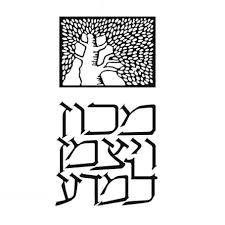
\includegraphics[width=1.2in]{Logo.png}}
% 	\fancyhead[R]{ 
\includegraphics[width=1.2in]{OpenLogo.jpg}}
}


%-----------------------------------------------------

%\title{Controlling a Superconducting Quantum Computer}
%\author{Daniel Cohen Hillel}
%\date{}

\begin{document}

\def\biblio{} % resets the biblio command, if not here a new reference list will be produced after every chapter

\begin{titlepage}
	
	\newgeometry{top=1 in, bottom=1 in, left=1 in, right= 1 in} 
	
	\thispagestyle{frontpage}
	
	\begin{center}
		
		\vspace*{6\baselineskip}
	
		
		{\Large \textbf{Controlling a Superconducting Quantum Computer\\}}
		
        \vspace*{1,5\baselineskip}

		\large{\textbf{Daniel Cohen Hillel}}\\
		\large{\textbf{Supervisor: Dr. Serge Rosenblum}}\\
		
		\vspace{1,5\baselineskip}
		
		\large{Advanced Project in Physics A (20382)}\\
		\large{The Open University of Israel}\\
		
		\vspace{1,5\baselineskip}
		\large{The Weizmann Institute}\\

	\end{center}
	
\end{titlepage}
\restoregeometry % restores the margins after frontpage
%\nocite{*} % uncomment if you want all sources to be printed in the reference list, including the ones which are not cited in the text 

\pagenumbering{gobble} % suppress page numbering
\thispagestyle{plain} % suppress header

%\maketitle

\newpage

\tableofcontents

\newpage
\pagenumbering{arabic}
\section{Introduction}
\subsection{What is a Quantum Computer?}
We'll assume the reader understands the basics of computing and quantum mechanics, here's a brief overview. \newline
 A classical computer is, essentially, a calculator, not of "Regular" numbers but of \textit{binary numbers}\footnote{ add further reading about binary numbers}. % TODO: <---
 A \textit{binary digit}("\textit{bits}" from now on) can be in one of two states, usually represented by 0 and 1. We can use \textit{logic gates} to control and manipulate bits to do all kinds of calculations\footnote{Additional information about bit calculation}. This is the building blocks of the classical computer, with the ability to do calculation with bits, and the ability to store bits in the memory we are able to construct a computer.
 
So what is a quantum computer then? Well, if the classical computer uses bits to do calculations, a quantum computer uses \textit{quantum bits}("\textit{qubits}" from now on) for it's calculations. A qubit, much the same as a bit, has 2 states, a 0 state and a 1 state(notated $\ket{0}$ and $\ket{1}$ for reasons we'll see later), the difference is that a qubit can be in a \textit{superposition} of the 2 states, we can use that property to our advantage to create new type of computation.

\subsection{Qubits and Quantum Gates}
Mathematically, we think of qubits as 2-dimensional vectors, where the first term corresponds to the $\ket{0}$ state and the second term corresponds to the $\ket{1}$ state, so a qubit in a state $\frac{1}{\sqrt{2}} \ket{0} + \frac{1}{\sqrt{2}} \ket{1}$ can be represented as
\[
\begin{pmatrix}
    \frac{1}{\sqrt{2}} \\
    \frac{1}{\sqrt{2}} 
\end{pmatrix} = \frac{1}{\sqrt{2}} \ket{0} + \frac{1}{\sqrt{2}} \ket{1}
\]
In this world of qubits as vectors, we think of logic gates, known as \textit{quantum gates}, as matrices\footnote{There is a requirement that the matrices will be unitary}, and when the qubit goes through the logic gate, the result is multiplying the matrix by the qubit. Let's see an example for one of the simplest logic gates we have in classical computing, the NOT gate, a quantum implementation of this gate will take $\ket{0}$ to $\ket{1}$ and $\ket{1}$ to $\ket{0}$), the matrix that achieves this is 
\[
\begin{pmatrix}
    0 & 1 \\
    1 & 0
\end{pmatrix}
\]
Also called $\sigma_1$\footnote{known as the Pauli matrix 1}. We can see that if we, for example, input a $\ket{0}$ into that quantum gate, we get as a result
\[
NOT \ket{0} = 
\begin{pmatrix}
    0 & 1 \\
    1 & 0
\end{pmatrix}
\begin{pmatrix}
    1 \\
    0
\end{pmatrix} = 
\begin{pmatrix}
    0 \\
    1
\end{pmatrix} = \ket{1}
\]
As we expected. There are many more 1-qubit quantum gates we can think of(infinite amount actually). The interesting thing is that in classical computing, we only have 4 possible logic gates on a single bit(compared to infinite amount for qubit), these are the identity(do nothing), the NOT, output always 1, and output always 0. % TODO: Horrible wording
The last thing we need to know to understand the basic of quantum computing, is how to treat multiple qubits. If we have sevral of qubits in our system, we think of all the qubits together as one vector that is the \textit{tensor product}\footnote{Kronecker product to be precise} of all the qubits, so let's say we have a $\ket{0}$ and $\ket{1}$ qubits in our system, we represent that by $\ket{01}$ and it is equal to
\[\ket{01} = \ket{0} \otimes \ket{1} =
\begin{pmatrix}
    0 \\
    1 \\
    0 \\
    0
\end{pmatrix}\]
And a quantum gate on multiple qubits is simply a larger matrix. 
The thing about the tensor product is that for N qubits, it has $2^N$ coefficients(!) % TODO: Make the reader excited about this or something, more is needed

Now that we have the basic tools of quantum computing, we can use them to get motivation for the amazing things quantum computers can do

\subsection{Algorithms and Further motivation}
% TODO: add the example of the black-box gate and lead to shor's algorithm(no actual explenation of the algorithm but explain that with some work you can get to it) to motivation the reader
...
\subsection{Superconducting Quantum Computers}  % TODO: Maybe put this under the "Our SYstem" chapter?
The physical implementation of the qubit itself isn't to subject of this project but we can look a bit on how you would implement such a thing. A problem we face when making a quantum computer is would physical phenomena would actually be the qubit. For classical computer we already have this figured out for years, the bit is the voltage on a wire, 1 is one there is voltage on the wire and 0 is if there's none, simple. For a quantum computer this is much more complicated, there are many quantum phenomena we can use as our qubit, such as the energy level of an atom, the spin of an electron, the polarization of photons and so on. This project is about a \textit{superconducting} quantum computer, with superconducting  qubits.

Superconducting qubits are microwave circuits in which the cooper-pair condensate effectively behaves as a one-dimensional quantized particle. By inserting Josephson junctions, the circuit can be made nonlinear, allowing us to isolate the qubit from higher-energy levels and treat it as a two  level system(instead of the many level system that it really is).
% TODO: This need to be built from the ground up and can't be all by the way-y. Need to ask Serge and read about superconductors a bit, look into BCS theory
% TODO: Need to explain much on superconductors and cooper pairs
% TODO: Much more to add
\newpage
\section{Our System}

\subsection{The cavity}

\subsection{The Transmon}

% \subsection{The Oscillator}

\subsection{Describing the System Mathematically}  % TODO: Mention the JC model
To describe the system mathematically we are going to calculate it's Hamiltonian, that way we can run simulations of the system with the Schrodinger equation.\par
We can partition the system into different parts and analyse each part individually, so the total system Hamiltonian will be:

\begin{equation}
H(t) = H_{Oscillator} + H_{Transmon}+ H_{Interaction} + H_{Drive}(t)
\end{equation}

We'll begin by the easy to characterize, Transmon And Oscillator, they are a simple quantum system that can be described by the uppering and lowering operators \footnote{See appendix A}. We can write:
\begin{equation}
H_{Oscillator} = \omega_C a^\dag{}a
\end{equation}
\begin{equation}
H_{Transmon} = \omega_T b^\dag{}b
\end{equation}
We can find $\omega_C$ and $\omega_T$ experimentally. % TODO: Maybe add a few words about how to do so and about the fact that this is only an harmonic approximation
\par
The next part to characterize is the interaction(See appendix A), by the Jaynes–Cummings model, we can write the interaction Hamiltonian as:
\begin{equation}
H_{Interaction} = \chi a^\dag{} a  b^\dag{} b % Again, this is only an harmonic approximation
\end{equation}
Again, we can measure $\chi$ experimentally.  % TODO: Maybe add more about how it's done
\par
Finally, we can characterize the driven and most important part of the system. It can be written as: % TODO: Add more about how do you get to that equation. Is it from Maxwell?
\begin{equation}
H_{Drive} = \epsilon_C(t)a + \epsilon_T(t)b + h.c.
\end{equation}
Or as(expanding the hermitian conjurgate):
\begin{equation}
H_{Drive} = \epsilon_{I_C}(t)(a + a^\dag{}) + \epsilon_{Q_C}(t)(a - a^\dag{})i + \epsilon_{I_T}(t)(b + b^\dag{})+ \epsilon_{Q_T}(t)(a - a^\dag{})i
\end{equation}
each \(\epsilon\) is a pulse that we will optimize with GRAPE as described in much details in the next chapter.

\newpage
\section{Optimal Control}

\subsection{What's GRAPE} % TODO: Add imagery of a step-wise constant function
As explained in previous sections, to control our qubit and manipulate it, we need to send microwave pulses in the cavity. The problem is, what pulse do we send? How does it look? sin? cos? In what frequency? or maybe even some arbitrary wave. \par
To answer this question, we can model our system on a normal computer and simulate what happens when you send a pulse, then, we can try to change the pulse(in a smart way) until we get the desired effect. So for example, let's say we want to find the wave pulse that corresponds to the NOT gate, we can start by guessing some random wave(constant zero, sin and so on), the random wave probably won't act as a NOT gate, then, we change the wave a little bit many times and on each iteration the pulse acts more and more as a NOT gate.\par
So what's GRAPE than? The *GR*adient *A*scent *P*ulse *E*ngineering was first proposed in [2]. When we model our system, we treat the wave as a step-wise constant function, so the wave is just an array with many variables and we want to find the best values that give the result that we want. then we set a cost function \footnote{discussed in details in the next section} that tells us how are the values of the wave to give the wanted result. This cost function is a many dimensional function(each step of the wave is a dimension of the cost function), and we can find its gradient. Using the cost function and it's gradient we can use some optimization algorithm(mainly, the L-BFGS-B method) to find the maximum of the cost function that gives us the optimal wave to send to the cavity.

\subsection{The Cost Function}
So what is this cost function really? \textit{\textbf{Fidelity}}. It measures the "closeness" of two quantum states and varies between 0 and 1. So for example, the fidelity between state $\ket{0}$ and state $\ket{1}$ is equal to 0, because they are the most different two quantum states can be, while for example the fidelity between state $\ket{0}$ and state $\ket{0}$ is equal to 1, because they are the closest two states can be to each other(for a matter of fact, every state has fidelity 1 with itself and end fidelity 0 with an opposite state). But still, how do we calculate the fidelity between two states? well, turns out its very simple, it's just their product \footnote{Assuming both states are pure states}. We can write:

\begin{equation} \label{def:fid}
F(\psi_1, \psi_2) = \abs{\braket{\psi_1}{\psi_2}}^2
\end{equation}
We want to maximize the fidelity with GRAPE.\par
In a previous chapter we characterized the Hamiltonian of the system(equation (num)), so now we can use the good old \textit{time-dependent Schrodinger equation}:

\begin{equation}
i\hbar\frac{d}{dt}\ket{\Psi(t)} = \hat{H}\ket{\Psi(t)}
\end{equation}

And also, the Hamiltonian of the system is in the form\footnote{Further details were given in section 2.4}:

% TODO: Add explanation about that there are multiple different pulses and throughout the chapter we're referring to a single pulse which is most of the time not the case
\begin{equation}
H(t) = H_0 + \sum_k{\epsilon_k(t) H_k} % Maybe put the next part before the part about the Schrodinger equation
\end{equation}

Because of the way this Hamiltonian is built, on each constant step of the wave function, the Hamiltonian is constant, and luckily for us, the solution of the Schrodinger equation for a constant Hamiltonian is pretty simple and given by\footnote{Add a simple justification} % TODO: Add justification

\begin{equation}
U(t) = e^{-\frac{i}{\hbar}\int_{T_0}^{T_1}H(t)dt}
\end{equation}

And because we chose $T_0$ and $T_1$ as the end points of a step of the functions, the total Hamiltonian of the system is constant so the integral is just a simple multiplication by $T_1-T_0$ which we'll write as $\delta t$. So the solution is
\begin{equation}
U(t) = e^{-\frac{i\cdot \delta t}{\hbar}H(t)}
\end{equation}
More then that, to solution over all time is the product of all the solutions for each constant piece. So 
\begin{equation}
U(\epsilon(t)) = \prod_{k = 1}^NU_k
\end{equation}
Where N is the number of time steps in the simulation(larger N is a more precise simulation). \par
This way the state of the qubit after the drive is given by:
\begin{equation}
\ket{\Psi_{final}} = U\ket{\Psi_{initial}}
\end{equation}
This way if we want to calculate the fidelity after applying the drives we can simply calculate the fidelity between the wanted state and the final state,
\begin{equation}
F(\Vec{\epsilon(t)}) = F(\Psi_{target}, \Psi_{final}) = \abs{\bra{\Psi_{target}}U\ket{\Psi_{initial}}}^2
\end{equation}

Now, theoretically we can use an algorithm to try different waves until we find a wave that does what we want(brute force for example), but this will take to much time and the computation won't finish in any reasonable amount of time. Because of this, we'll want to use a smart search algorithm(such as L-BFGS-B) but to do so we need the gradient of the cost function(the variables of the cost function are the values of the steps of the drive pulses). We can obviously use the finite difference method to calculate the gradient but this method is heavy on the computation and has a lot of over head. We'll take a smarter approach to calculating the gradient.\par
We can look at the expression,  % TODO: Need to go over this

\begin{equation} \label{def:overlap}
c = \braket{\Psi_{target}}{\Psi_{final}} = \bra{\Psi_{target}}U\ket{\Psi_{initial}}
\end{equation}

We want to differentiate this expression by each control parameter. U is defined as:

$$U = U_N U_{n-1}...U_2 U_1$$

And when differentiating by a control parameter only one $U_k$ is affected, so we can write,

$$\frac{dc}{d\epsilon_k} = \bra{\Psi_{target}}U_N U_{N-1} ... U_{k+1}\frac{dU}{d\epsilon_k} U_{k-1} ...U_2 U_1\ket{\Psi_{initial}} $$

We can write that for a constant Hamiltonian(from the schrodinger equation)
$$U_k = e^{-\frac{i\cdot \delta t}{\hbar}H(t)}$$
We can approximate the derivative $\frac{\partial U_k}{\partial \epsilon_k}$ in the limit of small $\delta t$ by writing
\begin{equation*}
    \frac{\partial U_k}{\partial \epsilon_k} \approx -\frac{i\cdot \delta t}{\hbar}\frac{\partial H}{\partial \epsilon_k} \cdot e^{-\frac{i\cdot \delta t}{\hbar}H(t)} = -\frac{i\cdot \delta t}{\hbar}\frac{\partial H}{\partial \epsilon_k} U_k
\end{equation*}

We can use this expression as the gradient values but it's still rather complex computationally($o(N^2)$ complexity).\par
We can use a bit different method to calculate the gradient to save on the computation by reducing the overhead.

Now the derivitive of the cost function by an amplitude of the wave has become
\begin{equation} \label{eq:cost_init_deriv}
    \frac{dc}{d\epsilon_k} = -\frac{i\cdot \delta t}{\hbar} \bra{\Psi_{target}}U_N U_{N-1}... U_{k+1}\frac{dH}{d\epsilon_k} U_{k} ...U_2 U_1\ket{\Psi_{initial}} 
\end{equation}

Let's define 2 wave wave functions $\psi_{bwd}$ and $\psi_{fwd}$, they will be the multiplication component before and after the derivative of H, so:
\begin{equation} \label{eq:cost-function-b/fwd}
    \frac{\partial c}{\partial \epsilon_k} =  -\frac{i\cdot \delta t}{\hbar}\bra{\psi_{bwd}^{(k+1)}} \frac{\partial H}{\partial \epsilon_k} \ket{\psi_{fwd}^{(k)}}
\end{equation}
We can easily see from \ref{eq:cost_init_deriv} that 
\[   
\ket{\psi_{fwd}^{(k)}} = 
     \begin{cases}
       \ket{\psi_{init}} &\quad\ k=0\\
       U_k \ket{\psi_{fwd}^{(k-1)}} &\quad\ otherwise\\
     \end{cases}
\]
\[   
\ket{\psi_{bwd}^{(k)}} = 
     \begin{cases}
       \ket{\psi_{targ}} &\quad\ k=N+1\\
       U_k^{\dag{}} \ket{\psi_{bwd}^{(k+1)}} &\quad\ otherwise\\
     \end{cases}
\]
Now all we need is to do $2N$ calculations in the beginning($N$ for $bwd$ and $N$ for $fwd$) then calculating the actual gradient is trivial multiplication from equation \ref{eq:cost-function-b/fwd}. This improves the computation complexity in an order of magnitude($o(N^2)$ to $o(N)$) and the memory complexity by is still in the same order of magnitude($o(N)$ to $o(3N)$).

It's important to note that $c$ is not the fidelity, but the overlap. We can get the fidelity from $c$ like so \footnote{See initial definitions of $c$ and the fidelity(\ref{def:overlap} and \ref{def:fid} respectively)}
\[
F = |c|^2
\]
since $c$ might be complex this derivative is a bit less trivial than it might look like. We can write $c(\vec{\epsilon})$ as $a(\vec{\epsilon}) + b(\vec{\epsilon})i$, where $a, b \in R$ and we get that 
\[
\frac{\partial F}{\partial \epsilon_k} = \frac{\partial |c|^2}{\partial \epsilon_k} = \frac{\partial ||a+bi|^2}{\partial \epsilon_k} = \frac{\partial (a^2 + b^2)}{\partial \epsilon_k} = 2(a\frac{\partial a}{\partial \epsilon_k} + b\frac{\partial b}{\partial \epsilon_k})
\]
We can notice that\footnote{$(\frac{\partial c}{\partial \epsilon_k})^*$ is the complex conjugate of the derivative of c} $c(\frac{\partial c}{\partial \epsilon_k})^* = a\frac{\partial a}{\partial \epsilon_k} + b\frac{\partial b}{\partial \epsilon_k} + (ab - \frac{\partial a}{\partial \epsilon_k}\frac{\partial b}{\partial \epsilon_k})i$, more importantly we can see that the real part of that expression is exactly what we need, putting it all into one formula we get
\begin{equation} \label{eq:fidelity_gradient_final}
    \frac{\partial F}{\partial \epsilon_k} = 2\cdot \Re{c(\frac{\partial c}{\partial \epsilon_k})^*}
\end{equation}
Now all you need is to plug \ref{eq:cost-function-b/fwd} and \ref{def:overlap} into \ref{eq:fidelity_gradient_final} and you got your gradient :)

\subsection{Constraints}
Having our simulation doing whatever it wants is nice and all but still unfortunally, we're living in the real world, and in the real world we can't just make ultra-fast frequencies at close to infinite power, it's just impossible because of the limitation of our devices. We need to add constraints to the cost function so we won't get solutions that use too much power or that change too rapidly.

We define a set of constraints on the solution ${g_i \ge 0}$(ideally $g_i=0$). We can associate a Lagrange multiplier $\lambda_i$ to each constraint. \newline
Now our goal is to maximize 
$$F(\vec{\epsilon}) - \sum_i \lambda_i g_i(\vec{\epsilon})$$
Let's add a constraint to each of the most problematic physical limitation
\subsubsection{Limiting the Pulse Amplitude}
This is the most obvious physical limitation, we can't generate pulses with infinite energy, so we have to restrict it. There are two ways we can do so, the first is to create a hard cut-of amplitude, no matter what, the amplitude will never go above this amplitude, this will usually be the limit of our pulse generator. But normally we don't want our generator to work at it's absolute limit\footnote{Not only that it might damage the device but also with stronger pulses the non-linear optics effects increase and then it's no fun :(}, so we can add also a soft amplitude maximum by "rewarding" the cost function to stay at a lower amplitude. Let's see how we would implement such a thing, starting with the hard cut-off.

Instead of controlling and changing the amplitude($\vec{\epsilon}$) directly, we'll introduce a variable $\vec{x}$ and relate them as
$$\vec{\epsilon} = \epsilon_{max}\tanh{\vec{x}}$$
As you properly guessed, $\epsilon_{max}$ is the maximum amplitude of the pulse.
Since the optimization algorithm can only change $\vec{x}$, the amplitude of the pulse will always be between $-\epsilon_{max}$ and $\epsilon_{max}$. Unluckily for us, this changes the gradient of the cost function since we now want the derivative with respect to $\vec{x}$ instead of $\vec{\epsilon}$. We can relate the two
\[
\frac{\partial F}{\partial \vec{x}} = \frac{\partial F}{\partial \vec{\epsilon}}\frac{\partial \vec{\epsilon}}{\partial \vec{x}} = \frac{\epsilon_{max}}{\cosh^2{\vec{x}}} \ \frac{\partial F}{\partial \vec{\epsilon}}
\]
We can use the derivative $\frac{\partial F}{\partial \vec{\epsilon}}$ we got from \ref{eq:fidelity_gradient_final} and simply calculate $\frac{\epsilon_{max}}{\cosh^2{\vec{x}}}$ and we again have the gradient.

For the soft limitation, there are two limitation we can make, linear and non-linear. The linear goal is for general preference of low amplitude pulses and the non-linear is if you have a specific \(\epsilon_{max,soft}\) that you want to be well below of(You can use both or either one depends on your desired pulse properties). We'll start with the linear case since it's simpler.

For the linear amplitude penalty all we want is that \textit{bigger amplitudes} \(\Rightarrow\) \textit{bigger cost function}, since our algorithm seeks to minimize the cost function, this will lead to the overall amplitude being smaller. The way we do so is simple, we can define a constraint \(g_{amp,lin}\) that sums all the amplitudes of the steps of the pulse, so
\[
    g_{amp,lin} = \sum_k |\epsilon_k|^2
\]
and we maximize the cost function as explained at the beginning of the section.

Still, since it is added to our cost function we need to find the gradient of the penalty as well. In the case it's rather simple since it's a basic parabola
\[
    \frac{\partial g_{amp,lin}}{\partial \epsilon_k} = 2\epsilon_k
\]
and now we have all we need in order to add this penalty to our cost function. Let's move on to the non-liner penalty.

For the non-linear amplitude penalty we have a slightly different goal in mind
% TODO: Add here


\subsubsection{Limiting the Pulse Bandwidth and Slope}
Again we encounter a physical limitation, we can't produce any pulse we want, there's a limitation of the maximum frequency our AWG(Arbitrary Waveform Generator) can create because the device can't change the voltage instantaneously. Again, like we had with the amplitude limit, there are 2 types of limits we can make, hard and soft. Let's start with the hard limit.

We have some frequency \( \omega_{max} \) which is the maximum frequency that our AWG can generate. To make sure that our simulation doesn't produce such a pulse we can go from time space to the frequency space with a Fourier transform(Discrete Fourier Transform to be exact).
\[
    \vec{\epsilon} = (DFT)^{-1} \vec{x}
\]
The numerical optimization algorithm controls \(\vec{x}\) which is in the frequency space. Now if we want to limit the frequency we can simply set to 0 any frequency that is above our maximum frequency.\footnote{Might be more efficient to set these frequency to 0 and not let the optimization algorithm to try to change them(living the completely out of the pulse then putting them back in as 0 after the optimization is finished)}
\[
    x(\omega > \omega_{max}) = 0
\]
The gradient of the new cost function is simply the Fourier transform of x
\[
    \frac{\partial \vec{x}}{\partial \epsilon_k} = (DFT) \frac{\partial \vec{\epsilon}}{\partial \epsilon_k}
\]
And we know \(\frac{\partial \vec{\epsilon}}{\partial \epsilon_k}\) from previous sections.
It's important to note that the hard cut-off of the amplitude and the hard cut-off of the frequency do not work together since one is in the time space and one is in the frequency space. This is not much of a problem since we can compensate with the soft limits that do work well together(mainly since they require adding to the cost function instead of changing coordinate). In my simulations I use the amplitude hard limit instead of the frequency one since it only requires "squishing" the function instead of going from time space to frequency space.

For the soft limits, we're limiting the slope(derivative) of the pulses and not the frequency directly. There are, again, two types of limits we can make, a linear limit and a non-linear limit. The linear limit simply incentives for a lower maximum slope overall, and the non-linear limit incentives a specific maximum soft limit on the slope, we can use the two together. Let's start with the simpler, linear limit.

The slope of a step function is simply \(\epsilon_{k+1} - \epsilon_{k}\), we want to limit the size of the slope so we'll look at the expression \(|\epsilon_{k+1} - \epsilon_{k}|^2\) instead. Summing all the slopes(to get an overall slope size of the entire pulse) we get the expression\footnote{Note that we have a problem at the edges since the slope of the end points is not well defined, we'll fix this problem later but for now we just ignore the last point \(k=N\)}
\begin{equation}\label{eq:g_slope,lin}
    g_{slope, lin} = \sum_{k=0}^{N-1} |\epsilon_{k+1} - \epsilon_{k}|^2
\end{equation}{}

Remember that for each limit we associate a number \(\lambda_{slope, lin}\) that is the "strength" of the limit, and that the cost function now becomes: \textit{*old cost function*} + \(\lambda_{slope, lin} g_{slope, lin}\), so we need to calculate the gradient of this limit and add it to the total gradient of cost function.

Unlike the amplitude, since the slope of the boundaries is not well defined we'll have the edges defined differently then the center of the pulse. The gradient of \(g\) in the center is a simple derivative, notice that each \(\epsilon_k\) appears only twice in the sum
\[
    \frac{\partial g_{slope, lin}}{\partial \epsilon_k} = 4\epsilon_k - 2(\epsilon{k+1} + \epsilon{k-1})
\]
It's nice to see that the expression looks like how'd you numerically estimate the second derivative, since the gradient of the slope(which is the derivative) is the second derivative, this is nice and reassuring :). Now we need to define the gradient at the edges, you can see that the derivative of \(\epsilon_k\) depends on his 
+neighbors on both sides, since the first and last element of the pulse don't have 2 neighbors they are treated a little differently. each of the edges appears only once in the sum \ref{eq:g_slope,lin} unlike the others that appear twice, we can simply take the derivative of that one term and get
\begin{align*}
    &\frac{\partial g_{slope, lin}}{\partial \epsilon_0} = 2(\epsilon_1 - \epsilon_0) \\
    &\frac{\partial g_{slope, lin}}{\partial \epsilon_N} = 2(\epsilon_N - \epsilon_{N-1})
\end{align*} % TODO: This definitely needs some changing!!!
And now the slope soft linear limit is defined and so is it's gradient.

Now, before we continue to the non linear limit, we'll add another small constraint that will also solve the problem of the slope at the boundaries(you can think of it as a sort of boundary condition). It might seem weird at first, but we want to pulse to zero-out at the edges(the amplitude of the first and last steps of the pulse being equal to 0), this is since our AWG device can't immediately start a pulse with some amplitude, it can't get from 0 to that amplitude instantaneously(for the same reason we limit the slope in the first place). This could be achieved by simply setting the first and last steps of the pulse and their gradient to 0.
\[
    \epsilon_0 = \epsilon_N = \frac{\partial \ Cost}{\partial \epsilon_0} = \frac{\partial \ Cost}{\partial \epsilon_N} = 0
\]
This solves the problem we were trying to solve we were having with the slope at the boundaries, since the gradient is 0 at the edges and does not depend on it's neighbors. We can move on to the non-linear limitation now.

As we mentioned earlier, the goal of the non-linear limitation is to get a specific wanted maximum slope instead of making the slope as small as possible, this is, like in the 
% TODO: Add here but more importantly change how is the goal of the non-linear limitation explained.

% \subsection{Adding the Cavity}
% \subsubsection{From Pure State to Density Matrix}
% When we want to describe a qubit-cavity system we need to go from pure states to density matrices(explained in more details in a moment). Unluckily for us, this means changing how we calculate the fidelity and it's gradients, so we'll need to change some of the equations we used in the previous section to get GRAPE to work in such a system.
% TODO: Need to add here alot, maybe change the wording
\subsubsection{Limiting the photon number} 
\centerline{\say{Hilbert space is a big place.}}
\centerline{-Name} % TODO: Add the name of who said it
Here's the thing about the cavity levels, there are infinite amount of them. This might be a problem since our computers can't really deal with infinite amount that well. We can make an assumption that the cavity only has \(N\) levels but it is still possible that something happens in the higher levels that may affect the physical result that we didn't include in the simulation. We want to limit that and make sure that everything interesting is contained in the \(N\) levels that we have


\subsection{Implementing Qubit Operations with GRAPE}

\subsubsection{DRAG - Imperfect Qubits}
When we did all of our calculation on the qubit we didn't include one detail, it's really hard to create one. In the way our qubits are implemented, there are actually more then 2 levels, it's not a 2 level system but we treat it as one since the higher levels are off-resonance\footnote{as explained in the beginning}, but still there's a chance some of the higher levels will get excited by our pulses or some other physical phenomena and we want to account for it. The way we can do so is with the Derivative Removal via Adiabatic Gate(DRAG) algorithm. The idea being we make the qubit in the simulation to be more then a 2 level system, change the Hamiltonian a little bit(as you'll see later) so it accounts for the off-resonance higher levels and use the same grape algorithm to optimize for the entire system and not only the lower 2 levels.
% TODO: Penalty on higher levels
% TODO: Definitely needs some rewording and expanding

% \subsection{Results and Pretty Graphs :)}
% \textit{Note: There is no quantum chip we can use to do the experiment, the result are of the numerical simulations.}
% \subsubsection{Preparing a Fock State in the Cavity}
% ...
% \subsubsection{Some Gates(?)}
% ...
\subsection{Implementing Cavity Operations}
...
\subsection{From States to Gates(?)}
% TODO: Explain how you would go from state-GRAPE to gate-GRAPE and maybe implement it?
\textit{*Maybe add here how to create a gate-GRAPE from the state-GRAPE*}


\newpage
\section{Controlling a Superconducting Quantum Computer} \label{chap:FPGA}
\subsection{Overview}
\subsection{The AWG}
Consider for a moment what we want to do with our microwave generator to control a qubit, we need to send a high frequency signal and change it by a really small amount compared to its frequency(sending a GHz signal and changing it by MHz, 3 orders of magnitude difference). We can't just take a wave generator that generates a 10GHz signal and tell it to change from 10GHz to 10.0001GHz because it won't be precise enough, and even if the frequency generator is good enough so that we can make really accurate changes to the frequency, we still want to have the wave interact with the quantum system and analyze the result so we also need a super-frequency-analyzer to understand what the hell is going on in the quantum system, not only that, we also want the frequency analyzer and generator to work together(matching the same input with the corresponding output of the system). Now that we understand what are some of the challenges working with such high frequencies, what can we do about it?

Well the solution is simple, we can take a high frequency wave(10GHz for example) and a lower frequency wave(1MHz for example) and mix them together \textit{somehow} to get a $10\text{GHz} + 1\text{MHz} = 10.0001\text{GHz}$ signal, and in the output of the quantum system we can simply un-mix the result to get back the 10GHz signal and some other signal(in the MHz) that can tell us something about the system.

That sounds all nice and good but how do we actually mix/un-mix 2 signals in that way and how can we control that proccess? That's where the IO-Mixer comes in, we'll look into them in just a moment, first we need to understand a regular mixer work.

\subsection{The Mixer}
The idea is simple, the mixer has 2 inputs and one output, when you enter 2 waves as an input, you get their product as the output(inputting for example $\cos(t)$ and $\cos(2t)$ will result in $\cos(t)cos(2t)$ at the output). We look more into mixers, couplers and their implementation in appendix \ref{appen:Mixers}.

We draw a mixer in a diagram like so,

\begin{figure}[H]
    \centering
    \caption{Ideal mixer in a diagram}
    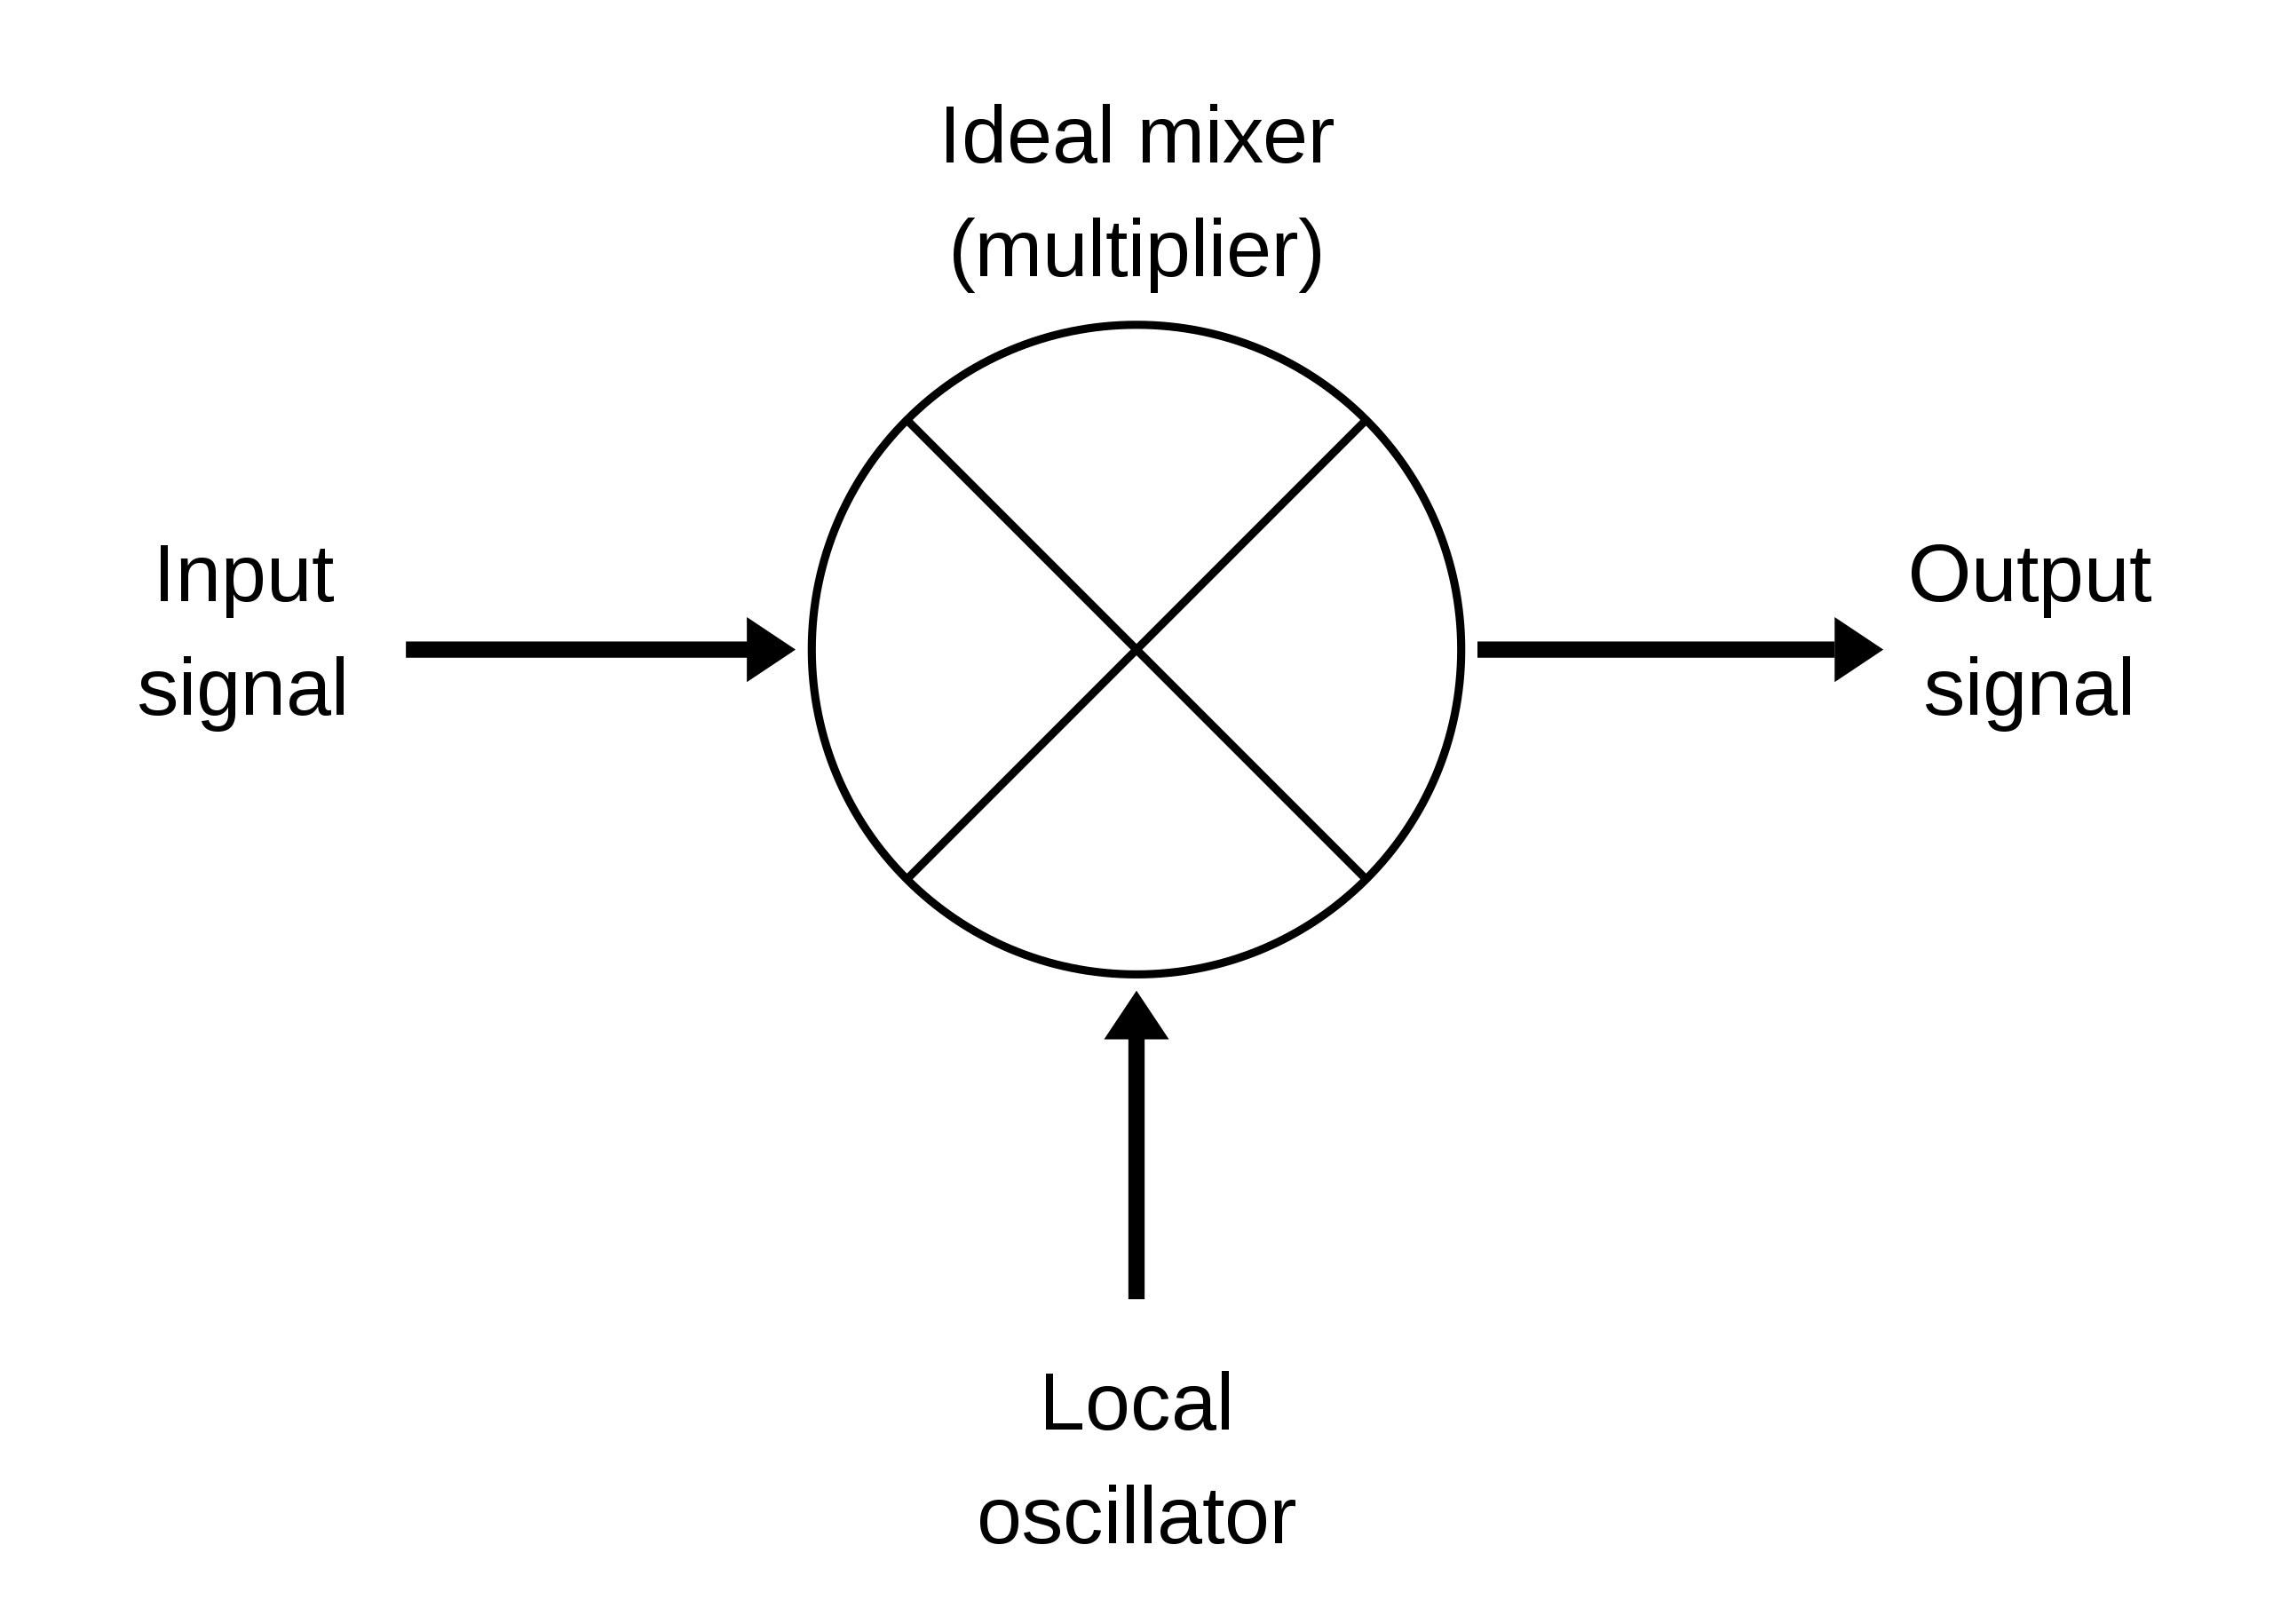
\includegraphics[width=0.3\columnwidth]{Ideal-Mixer.png} %TODO: Change image to one with L I R markings
    \label{fig:Ideal-Mixer}
\end{figure}
We can change what are the outputs and what are the inputs to get different ways for the mixer to work % TODO: Add on this later

\subsection{The IQ-Mixer}
% Marki website - sent on mail
We've seen what's a \textit{regular}(and \textit{ideal}) mixer is, but how can we use it for the desired effect? remember, we want to input a high frequency and a lower frequency and we want the output to be a wave with a frequency that is the sum of the 2 frequencies. To do so, we can consider the following diagram
\begin{figure}[H]
    \centering
    \caption{The IQ mixer}
    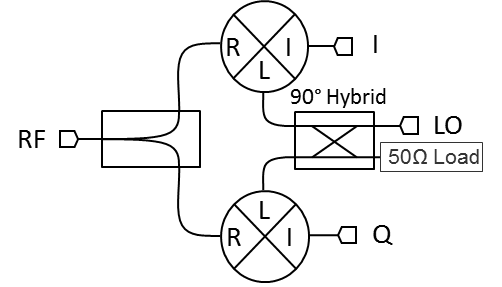
\includegraphics[width=0.5\columnwidth]{IQ-Mixer.png} %TODO: Change image to one with L I R markings
    \label{fig:IQ-Mixer}
\end{figure}
Where the \textit{90\degree hybrid} in the diagram is simply a 90\degree hybrid coupler, what it does is that it splits the signal to 2 waves at a 90\degree phase difference, we look into those in appendix \ref{appen:Mixers}. The square near the \textit{RF} sign simply adds the 2 waves, we also look into it in the appendix % TODO: Improve wording

As we can see, the IQ mixer has 3 inputs, \textit{I}, \textit{Q}(hence the name) and \textit{LO}. We can also see that there's only one output, \textit{RF}(although you can play with what are the inputs and what are the outputs).

How can we use this IQ mixer to add frequencies? Let's consider the following inputs\footnote{You can flip I and Q and get subtraction instead of addition}
\begin{align*}
    I &---> \cos(\omega_{IQ} t)\\
    Q &---> \sin(\omega_{IQ} t)\\
    LO &---> \sin(\omega_{LO}t)
\end{align*}
In this case, the input into the top mixer will be \textit{I} and a \textit{LO}, which is $\cos(\omega_{IQ}t)\sin(\omega_{LO}t)$. Similarly, the input into the bottom mixer will be \textit{Q} and 90\degree phase of \textit{LO}, which is $\sin(\omega_{IQ}t)\cos(\omega_{LO}t)$.

The total output(in \textit{RF}) will be the sum of the two waves
$$RF = \cos(\omega_{IQ}t)\sin(\omega_{LO}t) + \sin(\omega_{IQ}t)\cos(\omega_{LO}t)$$
and we know from simple trigonometry that $sin(a + b) = \cos(a)\sin(b) + \sin(a)\cos(b)$, so we get
\begin{equation}
    \boxed{RF = \sin((\omega_{LO} + \omega_{IQ})t)}
\end{equation}

Perfect! this is exactly what we wanted, the output is a wave with frequency that is the some of the input frequencies. Only one problem, it doesn't work :(.

\subsection{Theory VS Reality :(} % Maybe combine this section and the next one
What is the problem? We've proved mathematically that it should work, so why wouldn't it? The problem is that we can't just assume the waves to come and go with the same phase, the waves travel through the wire at some speed so if we input into two different wires, two waves that are at the same phase, at the other side of the wire they might come at different phases because of differences in wire length, resistance, etc... So what can we do about it? You could try to make identical parts and make everything just perfect but even slight deviation will cause the system no to work properly, a better solution is to input more complex waves and have some parameters to play with so we can simply find the right parameters for the system and then it will work.% TODO: Improve wording

We can analyze the frequency space of the output of out IQ mixer and we can see 2 types of it not working correctly
\begin{itemize}
  \item Leakage at the LO frequency
  \item Leakage at the harmonies($-\omega_{LO}, 2\omega_{LO}, 3\omega_{LO}, -2\omega_{LO}$...)
\end{itemize}
We can solve the first type of Leakage, at the LO frequency, by adding DC offsets to the input frequencies(We'll prove this mathematically later), and we can solve the second type of leakage by adding phase offsets to the waves(We'll prove this mathematically later).
This is how the frequency spectrum looks without making any changes to the input waves
%TODO: Add frequency space figure
\subsection{Solution for the real world} \label{sec:solution_real_world}
Let's consider now inputting into the IQ mixer the following waves instead of what we had earlier
\begin{align*}
    I &---> A_I\cos(\omega_{IQ} t + \phi_I) + \epsilon_I\\
    Q &---> A_Q\sin(\omega_{IQ} t + \phi_Q) + \epsilon_Q\\
    LO &---> \sin(\omega_{LO}t)
\end{align*}
Using the same calculation we did before, we get that
$$RF = I\cdot LO + Q\cdot LO(90\degree)$$
\begin{align}
RF &= (A_I\cos(\omega_{IQ} t + \phi_I) + \epsilon_I)\cdot \sin(\omega_{LO}t) + (A_Q\sin(\omega_{IQ} t + \phi_Q) + \epsilon_Q)\cdot \cos(\omega_{LO}t) \\
&=
\end{align}
\subsection{Finding Optimal Constants} % Maybe I won't do this section
As we've seen in the previous section, there are 4 variables we can "play" with to get the best variables for our system, as long as we don't change the system, these variables stay the same. What we want to do now is to actually find them. Our system is connected like so
% Add figure of how the system is connected

We have the Quantum Machine\footnote{this is the heart of the system, for now we'll use it to make the MHz waves with different phases, DC offsets and frequencies} that generates the I and Q inputs that go into the mixer(and also to an oscilloscope for debugging). There's the frequency generator\footnote{KeySight N5173B} that is connected to the mixer and generates 7GHz wave, and there's the frequency spectrum analyzer\footnote{SignalHound USB SA-124B} that is connected to the computer.

Let's first attack the leakage at the LO frequency. For now we'll have an LO frequency of 7GHz that we want to change by 25MHz(The same variables work for all frequencies this is just as an example)

\subsubsection{LO frequency Leakage}
As proven in section \ref{sec:solution_real_world}, to minimize this kind of leakage all we need is to play with the DC offsets of the IQ inputs. To do so, we first need to define what we want to minimize, which in this case is simply the power of the frequency at 7GHz, we can measure that power with our spectrum analyzer, we'll call that our \textit{cost function}.
We have a 2-dimensional variable space, we need to find where in this space the cost function is at a minimum. To do so, we'll start by using a brute force method to find the general location of the minimum in the variable space, since brute force is very inefficient we can't really use it to find the exact location of the minimum so we start by only doing a low precision brute force and then use a different optimazition algorithm to find the exact location of the minimum. We'll use the \texttt{scipy.optimize.fmin} as the algorithm for precise minimum location.\footnote{see more in appendix \ref{appen:opt}} % TODO: Improve wording
% TODO: Add figure of spectrum after leakage optimazation

\subsubsection{Harmonies Leakage}
Now that we've minimized the LO frequency leakage, we want to minimize the harmony leakage, we do that by changing to phases of the IQ waves from the quantum machine, it's important that changing the phases doesn't change the LO leakage and luckily for us, as proven in section \ref{sec:solution_real_world} that's whats happening. to change the phases we don't simply specify the phases, we use the correction matrix of the Quantum Machine. % TODO: Add explanations about the correction matrix(scale on angle) 
This time our cost function is the frequency at $\omega_{LO} - \omega_{IQ}$, we can do the same as we did in the LO leakage and use first a brute force optimization to find the general location of the minimum and the use the fmin algorithm to find the exact location of the minimum of the cost function(this time in the scale-angle variable space). You can see the result here
% TODO: Add figure of full final optimization
% TODO: Explain why it doesn't work perfectly(The quantum machine power problem)

\newpage
\section{Future Work and Conclusions}
...

\newpage

\appendix
\section{The Jaynes–Cummings Model}
Our goal is to mathematically model the Hamiltonian of a system of a two-level atom interacting with a single quantized mode of an optical cavity's electromagnetic field. % TODO: Add details about the original paper by Edwin Jaynes and Fred Cummings
\par
First we'll divide the system into 3 parts, The atom(it can be other two-level quantum systems), the cavity(electromagnetic field with quantized modes) and the interaction between the atom and the cavity(an atom can emit a photon to the cavity and change it's electromagnetic field, or catch a photon from the cavity and go up an energy level).\par  % http://aliramadhan.me/files/jaynes-cummings-model.pdf
Let's start with the cavity(we'll consider a one dimensional cavity for now). 
\subsection{The Homogeneous Electromagnetic Wave Equations}
Maxwell's equations in free space are:
\begin{subequations}
    \label{eq:optim}
    \begin{align}
        &\grad \cdot \textbf{E} = 0 \label{eq:Maxwell-1}\\
        &\grad \cdot \textbf{B} = 0 \label{eq:Maxwell-2}\\
        &\grad \cross \textbf{E} = \frac{\partial\textbf{B}}{\partial t} \label{eq:Maxwell-3}\\
        &\grad \cross \textbf{B} = \mu_0 \epsilon_0 \frac{\partial\textbf{E}}{\partial t} \label{eq:Maxwell-4}
    \end{align}
\end{subequations}
Taking the curl of \ref{eq:Maxwell-3} and \ref{eq:Maxwell-4} we get
\begin{subequations} 
\label{eq:curl-}
    \begin{align}
        &\curl{(\curl{\textbf{E}})} 
        = \curl{(-\frac{\partial \textbf{B}}{\partial t})} 
        = -\frac{\partial}{\partial t}(\curl{\textbf{B}})
        = - \mu_0 \epsilon_0 \frac{\partial^2 E}{\partial t^2} 
        \label{eq:curl-E}\\
        &\curl{(\curl{\textbf{B}})} 
        = \curl{(\mu_0 \epsilon_0 \frac{\partial E}{\partial t})} 
        = \mu_0 \epsilon_0\frac{\partial}{\partial t}(\curl{E}) 
        = - \mu_0 \epsilon_0 \frac{\partial^2 \textbf{B}}{\partial t^2} 
        \label{eq:curl-B}
    \end{align}
\end{subequations}
   
We can use the vector identity
\begin{equation}
    \nabla \times \left( \nabla \times \mathbf{V} \right) = \nabla \left( \nabla \cdot \mathbf{V} \right) - \nabla^2 \mathbf{V}
\end{equation}
And obtain from \ref{eq:curl-E} and \ref{eq:curl-B}
\begin{subequations}
    \begin{align}
        &\nabla(\nabla \cdot \textbf{E}) - \nabla^2 \textbf{E} 
        = -\mu_0\epsilon_0\frac{\partial^2 \textbf{E}}{\partial t^2} \\
        &\nabla(\nabla \cdot \textbf{B}) - \nabla^2 \textbf{B} 
        = -\mu_0\epsilon_0\frac{\partial^2 \textbf{B}}{\partial t^2}
    \end{align}
\end{subequations}
Now, we can use \ref{eq:Maxwell-1} and \ref{eq:Maxwell-2} To cancel the left most term and get
\begin{subequations}
    \begin{align}
        &\nabla^2 \textbf{E} = \mu_0\epsilon_0\frac{\partial^2 \textbf{E}}{\partial t^2}\\
        &\nabla^2 \textbf{B} = \mu_0\epsilon_0\frac{\partial^2 \textbf{B}}{\partial t^2}
    \end{align}
\end{subequations}
Now because we know that $v_{ph} = \frac{1}{\sqrt{\mu_0\epsilon_0}}$ and that the phase velocity of electromagnetic waves in a vacuum is the speed of light, $c_0$, we get
\begin{equation} \label{eq:Homo_electro_wave}
    \begin{split}
        \nabla^2 \textbf{E} = \frac{1}{c_0^2}\frac{\partial^2 \textbf{E}}{\partial t^2} \\
        \nabla^2 \textbf{B} = \frac{1}{c_0^2}\frac{\partial^2 \textbf{B}}{\partial t^2}
    \end{split}
\end{equation}
% TODO: Check these equations with serge
These equation are called \textit{the homogeneous electromagnetic wave equations}.
We'll pick a polarization arbitrarily to be in the x direction(that way we get only the component of the electric field and the y component of the magnetic field, $E_x$ and $B_y$) so now we get,
\begin{equation} \label{eq:Homo_electro_wave_pol}
    \begin{split}
        \frac{\partial^2 E_x}{\partial x^2} = \frac{1}{c_0^2}\frac{\partial^2 E_x}{\partial t^2} \\
        \frac{\partial^2 B_y}{\partial y^2} = \frac{1}{c_0^2}\frac{\partial^2 B_y}{\partial t^2} 
    \end{split}
\end{equation}
\subsection{The Hamiltonians}
We want to separate the total Hamiltonian into approachable parts, we can separate it like so,
\[
    H = H_{atom} + H_{cavity} + H_{interaction}
\]
where the atom and cavity Hamiltonians are the Hamiltonian of the atom and cavity if they were the only part of the (closed)system and the interaction Hamiltonian is the Hamiltonian of the interaction between the atom and the cavity in the system.

\subsubsection{cavity}

We can easily solve \ref{eq:Homo_electro_wave_pol} using separation of variables,
$$E_x(z, t)= Z(z)T(t)$$
Yielding the solution,
\begin{equation}
    \begin{split}
        E_x(z, t) = \sqrt{\frac{2 \omega_c^2}{V \epsilon_0}}q(t)\sin{kz} \\
        B_y(z, t) = \sqrt{\frac{2 \mu_0}{V}}\dot{q}(t)\cos{kz}
    \end{split}
\end{equation}
where $V$ is the effective volume of the cavity, $q$ is a time-dependent amplitude with units of length, and $k = m\pi/L$ for
an integer $m > 0$

The Hamiltonian is given by
\begin{align}
    H &= \frac{1}{2}\int\epsilon_0 \textbf{E}^2 + \frac{\textbf{B}^2}{\mu_0} dV \\
    &= \frac{1}{2}\int\epsilon_0 E_x^2(z, t) + \frac{B_y^2(z, t)}{\mu_0} dz \\
    &= \frac{1}{2}[\dot{q}^2(t) + \omega_c^2 q^2(t)]
\end{align}
This looks like the Hamiltonian of an harmonic oscillator.

Now, going from dynamical variables to operators(considering $\dot{q} \equiv p$) we get,
\begin{align}
     &\hat{E}_x(z, t) = \sqrt{\frac{2 \omega_c^2}{V \epsilon_0}}\hat{q}(t)\sin{kz} \\
     &\hat{B}_y(z, t) = \sqrt{\frac{2 \mu_0}{V}}\hat{p}(t)\cos{kz} \\
     &\hat{H} = \frac{1}{2}[\hat{p}^2(t) + \omega_c^2 \hat{q}^2(t)]
\end{align}

Let’s introduce creation and annihilation operators,
$$\hat{a}(t) = \frac{1}{\sqrt{2\hbar\omega_c}}[\omega_c\hat{q}(t) + i\hat{p}(t)]$$
$$\hat{a}^\dag(t) = \frac{1}{\sqrt{2\hbar\omega_c}}[\omega_c\hat{q}(t) - i\hat{p}(t)]$$

We can write the electric and magnetic field as,
\begin{align}
         &\hat{E}_x(   z, t) = E_0[\hat{a}(t) + \hat{a}^\dag(t)]\sin{kz} \\
         &\hat{B}_y(z, t) = \frac{E_0}{c}[\hat{a}(t) - \hat{a}^\dag(t)]\cos{kz}
\end{align}
And we can write the Hamiltonian as,
\begin{equation}
    \boxed{\hat{H}_{cavity} = \hbar\omega_c[\hat{a}\hat{a}^\dag + \frac{1}{2}] \approx \hbar\omega_c\hat{a}\hat{a}^\dag}
\end{equation}
We can ignore the zero-point energy $\frac{\hbar\omega_c}{2}$ if we define it as the zero energy point.

\subsubsection{atom}

Now that we have the cavity's Hamiltonian, we can go on to calculate the atom(qubit) Hamiltonian. \newline
Remember that the qubit is a 2-level system, meaning we can define it has a superposition of the ground, $\ket{g}$, and excited, $\ket{e}$, states. The energy of the atom is the sum of the energy of each state times it's energy($\sum E_sP(\ket{s})$). The probability to be in a state $\ket{s}$ is given by $\ket{s}\bra{s}$ so we can write,
\begin{equation}
    \hat{H}_{atom} = E_g\ket{g}\bra{g} + E_e\ket{e}\bra{e}
\end{equation}
Using the vector representation of these states we'll write,
%\begin{equation}
    \begin{align*} 
        \hat{H}_{atom} &= 
        E_e \begin{bmatrix}
        1 & 0     \\
        0   & 0   \\
        \end{bmatrix}
        + E_g \begin{bmatrix}
        0 & 0     \\
        0   & 1   \\
        \end{bmatrix} = 
        \begin{bmatrix}
        E_e & 0     \\
        0   & E_g   \\
        \end{bmatrix} \\
        &= \frac{1}{2}\begin{bmatrix}
        E_g + E_e & 0          \\
        0         & E_g + E_e  \\
        \end{bmatrix} +
        \frac{1}{2}\begin{bmatrix}
        E_e - E_g & 0          \\
        0         & -(E_e - E_g)  \\
        \end{bmatrix} \\
        &= \frac{1}{2}(E_g + E_e)\begin{bmatrix}
        1 & 0          \\
        0         & 1  \\
        \end{bmatrix} +
        \frac{1}{2}(E_e - E_g)\begin{bmatrix}
        1 & 0          \\
        0         & -1  \\
        \end{bmatrix} \\
        &= \frac{1}{2}(E_g + E_e)\mathbb{I} + \frac{1}{2}(E_e - E_g)\hat{\sigma}_z
    \end{align*}
%\end{equation}
Again, we can define the zero point energy so that the first term becomes $0$. We know the difference between the excited state energy and the ground state energy because it's approximately an harmonic oscillator so $E_e - E_g = \hbar\omega_a$ where $\omega_a$ is the atom frequency. Now we can write,
\begin{equation}
    \boxed{\hat{H}_{atom} = \frac{1}{2}\hbar\omega_a\hat{\sigma}_z}
\end{equation}

\subsubsection{interaction}

Now for the last part of the Hamiltonian, we want to know the interaction Hamiltonian between the atom and the cavity. The interaction Hamiltonian is now 
\[
\hat{H}_{interaction} = -\hat{\textbf{d}}\cdot\hat{\textbf{E}} = -\hat{d} E_0 \sin{kz} (\hat{a} + \hat{a}^\dag{})
\]
Where we introduced $\hat{d} = \hat{\textbf{d}} \cdot \hat{x}$ (remember that we defined the axis so that x is the direction of polarization of the electromagnetic field).
We'll also introduce the atomic transition operators
\[
    \hat{\sigma}_+ = \ket{e}\bra{g}, \quad\quad \hat{\sigma}_- = \ket{g}\bra{e} = \hat{\sigma}_+^{\dag{}}
\]
and the inversion operator
\[
\hat{\sigma}_3 = \ket{e}\bra{e} - \ket{g}\bra{g}
\]
only the off-diagonal elements of the dipole operator are nonzero so we may write
\[
    \hat{d} = d\ket{e}\bra{g} + d^* \ket{g}\bra{e} = d\hat{\sigma}_- + d^* \hat{\sigma}_+ = d(\hat{\sigma}_+ + \hat{\sigma}_-)
\]
thus the interaction Hamiltonian is
\begin{equation}
    \hat{H}_{interaction} = \hbar\lambda(\hat{\sigma}_+ + \hat{\sigma}_-)(\hat{a} +  \hat{a}^\dag) 
    = \hbar\lambda(\hat{\sigma}_+\hat{a} + \hat{\sigma}_+\hat{a}^\dag + \hat{\sigma}_-\hat{a} + \hat{\sigma}_-\hat{a}^\dag) 
\end{equation}
We shown the the operators $\hat{a}$ and $\hat{a}^\dag{}$ evolve as
\begin{equation}
    \hat{a}(t) = \hat{a}(0)e^{-i\omega t}, \quad\quad \hat{a}^\dag{}(t) = \hat{a}^\dag{}(0)e^{i\omega t}
\end{equation}
And similarly we can show for the free-atomic case that
\begin{equation}
    \hat{\sigma}_{\pm}(t) =   \hat{\sigma}_{\pm}(0)e^{\pm i\omega t}
\end{equation}
We can write while approximating $\omega_0 \approx \omega$
\begin{equation}
    \begin{split}
        &\hat{\sigma}_+\hat{a} \sim e^{i(\omega_0 - \omega)t}\\
        &\hat{\sigma}_-\hat{a}^\dag \sim e^{-i(\omega_0 - \omega)t}\\
        &\hat{\sigma}_+\hat{a}^\dag \sim e^{i(\omega_0 + \omega)t}\\
        &\hat{\sigma}_-\hat{a} \sim e^{-i(\omega_0 + \omega)t}
    \end{split}
\end{equation}
We can see that the last two term vary much more rapidly than the first two. Furthermore, the last two terms do not conserve energy(They correlate to [photon addition + atom excitation] and [photon reduction + atom grounded]), we're going to drop the last two terms and finally get
\begin{equation}
    \boxed{H_{interaction} = \hbar\lambda(\hat{\sigma}_+\hat{a} + \hat{\sigma}_-\hat{a}^\dag)}
\end{equation}

\par

Finally, we can write the full JC Hamiltonian
\begin{equation}
    \boxed{\hat{H} = \frac{1}{2}\hbar \omega_0\hat{\sigma}_3 
                     + \hbar \omega \hat{a}^\dag \hat{a} 
                     +  \hbar\lambda(\hat{\sigma}_+\hat{a} + \hat{\sigma}_-\hat{a}^\dag)}
\end{equation}
\subsection{Effective Hamiltonian in the Dispersive Limit}
...
% TODO: add derivation from "Introduction to Quantum Optics"

\newpage
%Examples of mixers and couplers
\section{Couplers and Mixers(?)} \label{appen:Mixers} % Maybe I'll get rid of this section entierly
Our goal here is to understand some ways you could physically implement some of the components in chapter \ref{chap:FPGA}, there are a lot of ways to implement each component but we're going to look at only a few. First we'll look into how would you implement a mixer, and then we'll see how would you implement a coupler(to make a phase difference).
\subsection{Single-Ended Diode Mixer}
\subsection{Single-Ended FET Mixer}
\subsection{Ring Modulator}
\subsection{Branch-Line Quadrature(90\degree) Coupler}
\subsection{Rat-Race Coupler}

\newpage
\section{Codes} \label{appen:Codes}
\subsection{IQ Mixer Optimization}
\subsection{GRAPE}
\subsection{Transmon-Cavity GRAPE}

\newpage
\section{Optimization Algorithms(?)} \label{appen:opt}
\subsection{fmin}
\subsection{L-BFGS-B}

\newpage
% TODO: Properly need to change this completely :(
\begin{thebibliography}{9}
    \bibitem{QuTIP} 
        J. R. Johansson, P. D. Nation, and F. Nori: "QuTiP 2: A Python framework for the dynamics of open quantum systems.", Comp. Phys. Comm. 184, 1234 (2013) [DOI: 10.1016/j.cpc.2012.11.019].
     
    \bibitem{einstein} 
        Albert Einstein. 
        \textit{Zur Elektrodynamik bewegter K{\"o}rper}. (German) 
        [\textit{On the electrodynamics of moving bodies}]. 
        Annalen der Physik, 322(10):891–921, 1905.
     
    \bibitem{knuthwebsite} 
        Knuth: Computers and Typesetting,\\
        \texttt{http://www-cs-faculty.stanford.edu/\~{}uno/abcde.html}
\end{thebibliography}

\end{document}


